\chapter{Equalizer GPU Implementation}
In Chapter \ref{chap:eq_eq} the equalizer equations were conditioned for GPU implementation.
This Chapter explains how the equalizers were implemented into GPUs.
Block diagrams will be the main tool here because the code is too nasty to show a simple example.

Before we jump into the explination of the equalizer implementation, we need to talk about a few things, namely Batched Processing in CUDA and convolution in GPUs.


\section{CUDA Batched Processing}
Typically when batched processing, each batch is ran independent of other batches.
In CPU this is done by calling the same function on different data.
Shouldn't GPUs be able to do the same thing...but in parallel.

CUDA has many libraries that are ``batched,'' meaning a GPU kernel launched for each batch of data.
Examples of using a batched libraries that are used in PAQ are cuFFT, cuBLAS and cuSolver.
Each of these libraries have batched kernels.
Figure \ref{fig:matrix_batch_vs_batched} shows the concept of a batched matrix multiply.
\begin{figure}
	\caption{Diagram showing the relationships between $z(n)$, $\rho(n)$ and $b(n)$.}
	\centering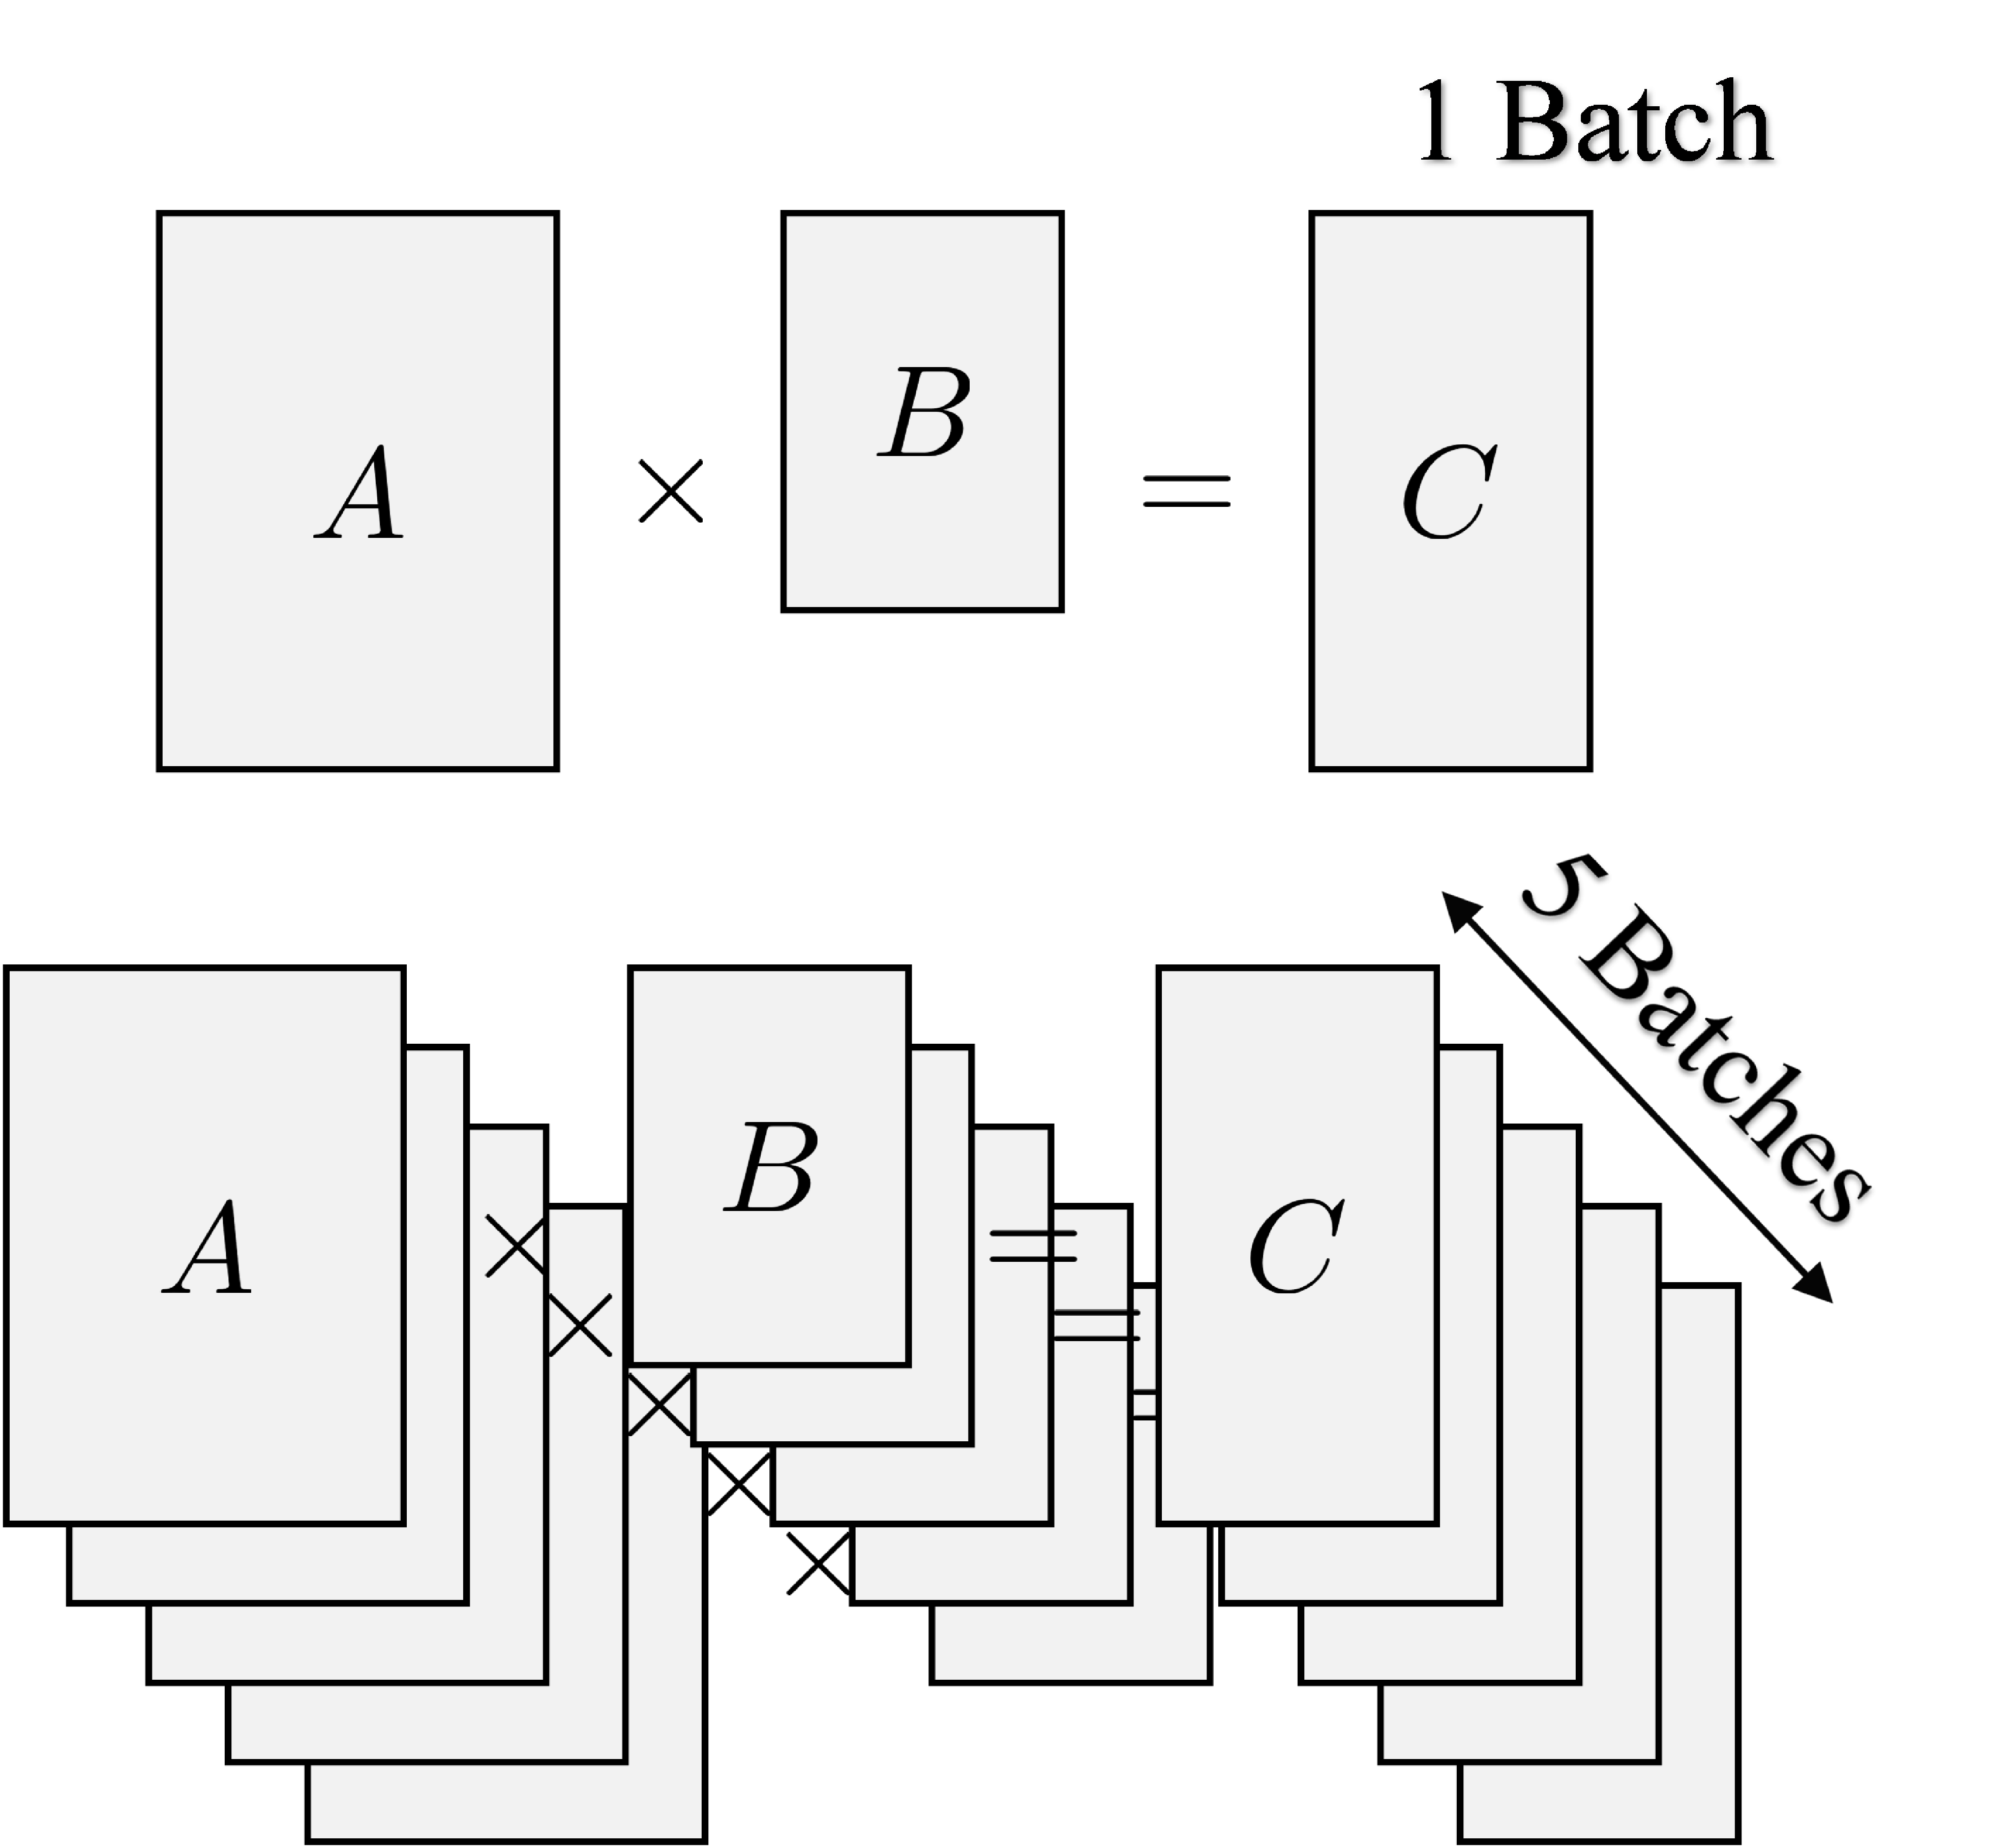
\includegraphics[width=4.13in/100*55]{figures/eq_GPUimplementation/matrix_batch_vs_batched.pdf}
	\label{fig:matrix_batch_vs_batched}
\end{figure}

Batched libraries perform much better than calling a GPU kernel multiple times with independent data.
Haidar et al. showed batched libaries in GPUs achive more Gflops per second than calling GPU kernels multiple times \cite{haidar2015optimization}.
Batched processing performs very well in GPUs because it increases parallelism, gives more opportunities for NVIDIA engineers to optimize and reduces overhead on the CPU.
The bottom line is use batched libraries as often as possible.

The PAQ system is suited very well for batched processing.
Each $1.907$ second set has $3104$ packets or batches of data as shown in Figure \ref{fig:packet_batch_set}.
If an operation is done on each packet, available CUDA batched libraries should always be used.
For simplicity, every block diagram shown in this chapter only applies to a single batch.
Every block diagram is batched and applied to $3104$ iNET packets.
\begin{figure}
	\caption{Diagram showing the relationships between $z(n)$, $\rho(n)$ and $b(n)$.}
	\centering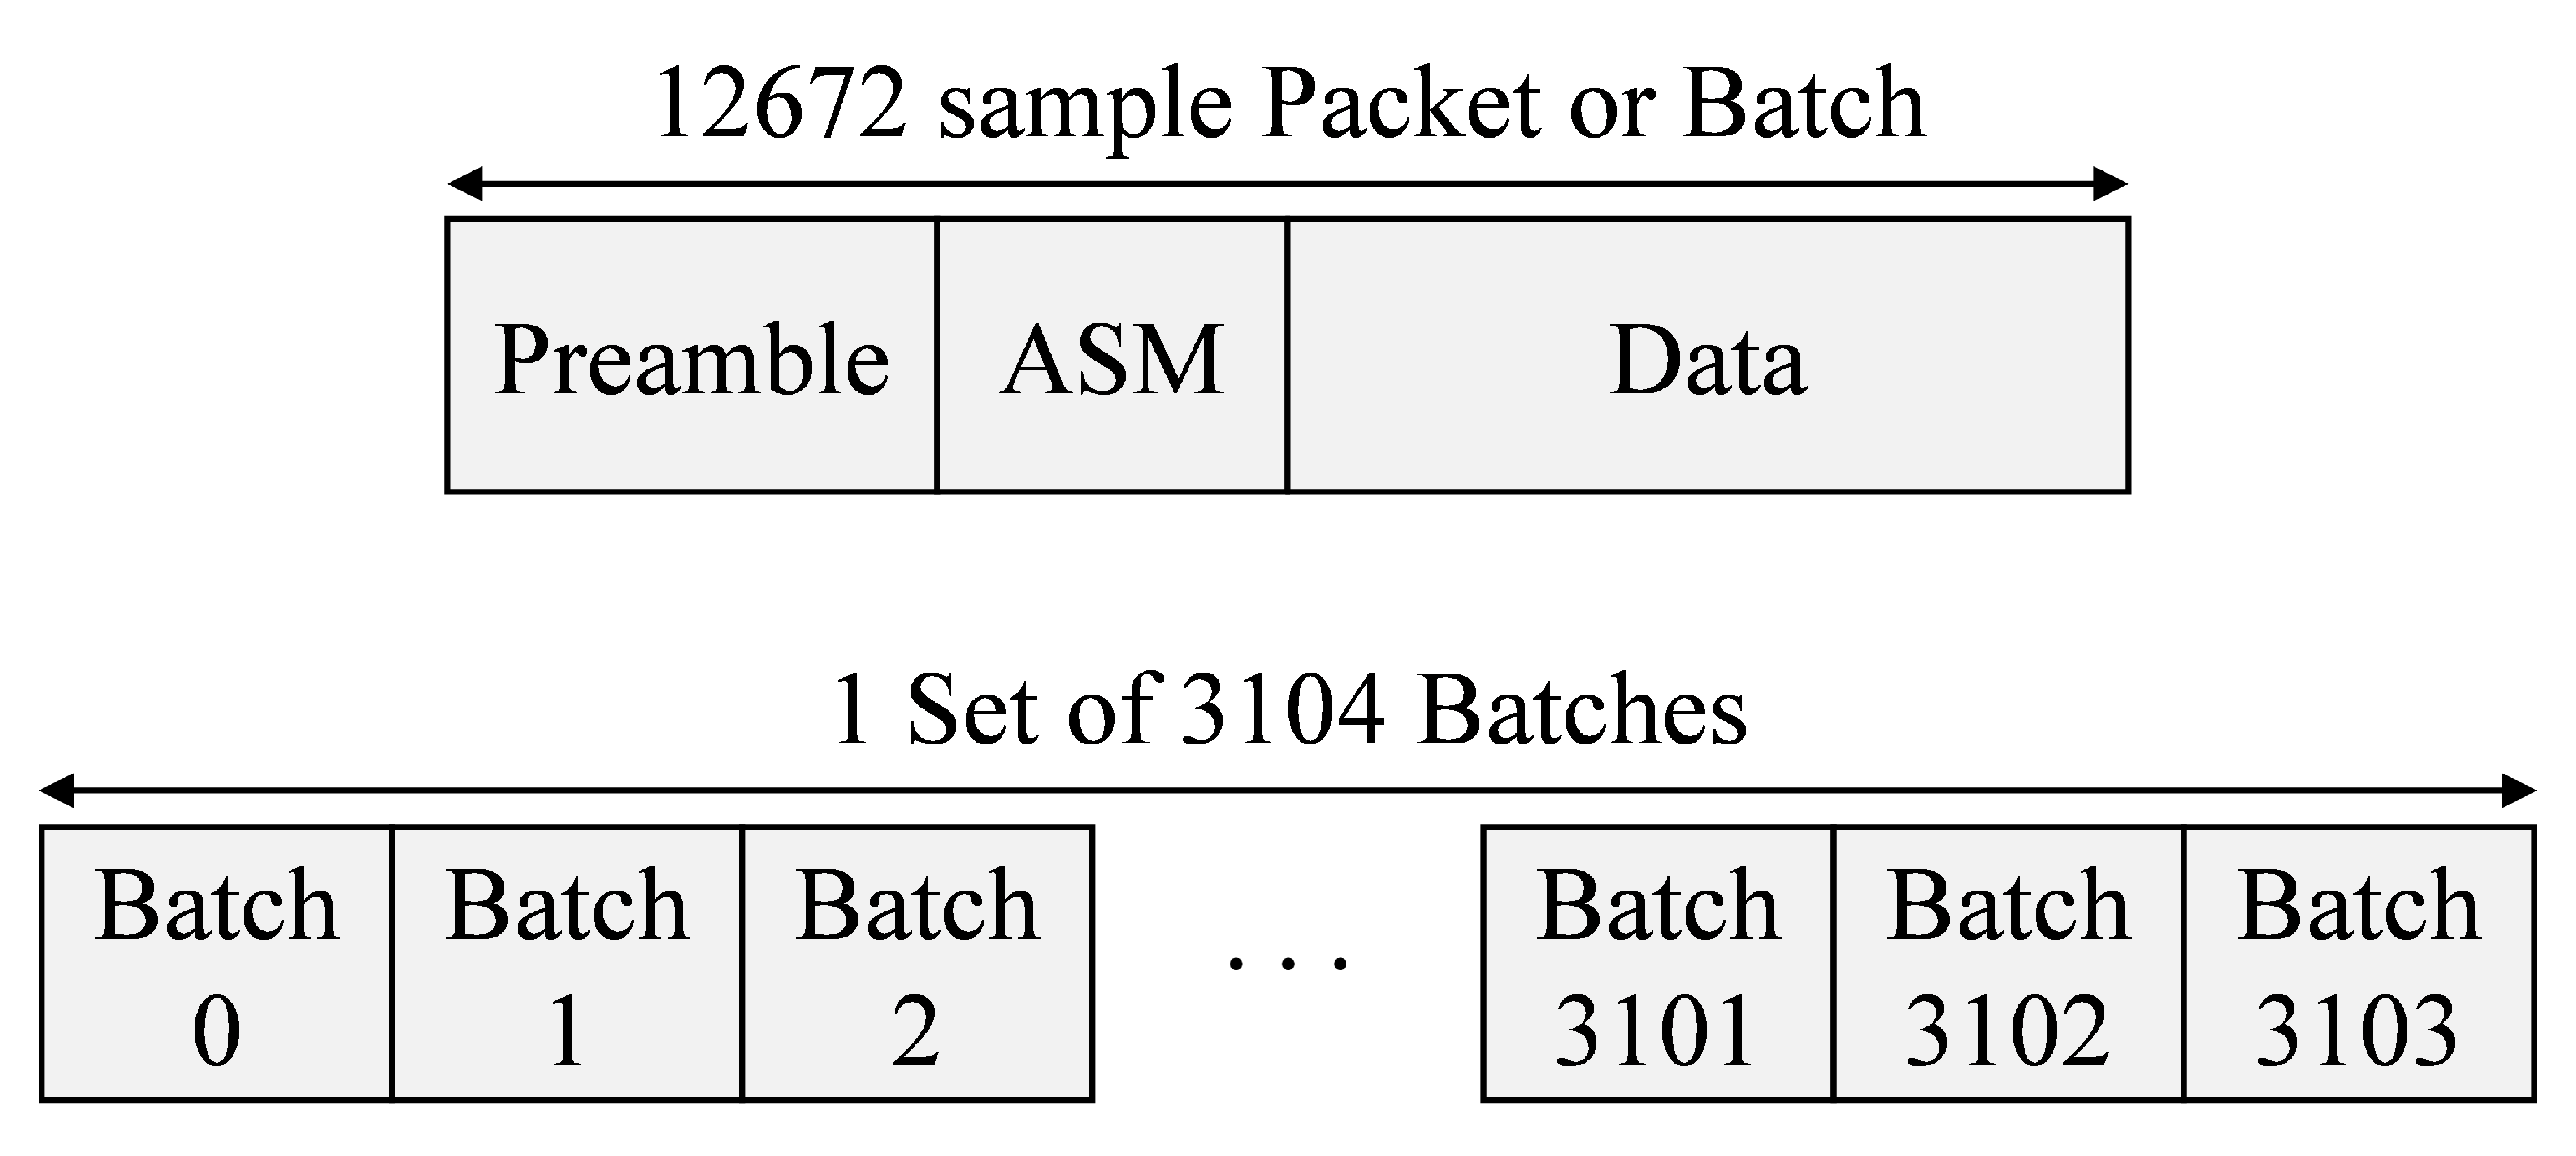
\includegraphics[width=5.94in/100*55]{figures/eq_GPUimplementation/packet_batch_set.pdf}
	\label{fig:packet_batch_set}
\end{figure}


\section{Batched Convolution}
Chapter \ref{chap:gpu} delved into comparing a single convolution in CPUs and GPUs in the time domain or frequency domain.
As talked about in Chapter blah, system overview, We dont only have a packet or batch, we have $3104$ packets or batches.
When we perform convolution we convolve $3104$ signals with $3104$ filters.
So...
How does the problem change?
Obviously doing batched convolution in a CPU will not be feasible and wont be considered.

Lets stay in GPU land.
Should we do convolution in the time domain or the frequency domain?
Are there draw backs to staying in the time domain? 
If we do convolution in the time domain, should we use shared memory?
Are there draw backs for going to the frequency domain? 

Get timing of convolution in the time domain global, time domain shared, time domain frequency.

There is one very important thing we have over looked...
We are doing just one convolution...we are doing two.
We have to convolve with the equalizer AND the numerically optimized detection filter $\mathbf{h}_{NO}$.
If we stay in the time domain, we have to do two cascaded convolutions.
Two convolutions takes...twice the time....
If we go to the frequency domain, the point to point or hadamard product is done with 3 inputs rather than 2.
Convolving with 2 inputs vs even 10 inputs is about the same.
The only required part is performing the FFT on the inputs and performing the $N$ way multiply...

Well, $\mathbf{h}_{NO}$ doesn't change, so we compute the FFT of the detection filter $\mathbf{H}_{NO}$ and store it.
So doing the convolution requires taking the FFT of 2 vectors $\mathbf{c}$ and $\mathbf{r}$.
After the hadamard product, the functions independent of how many filters we are convolving with accept for we may have to trip off different parts depending on what we are convolving with.

Optimizing convolution speeds up every equalizer because every equalizer uses convolution...CMA uses convolution twice per iteration. 

\section{Equalizer Implementations}
Until now every all equations and block diagrams explain processing one packet of data.
In the PAQ system, each batch of data has $3103$ or $3104$ packets in the $39321600+12671$ samples.
Each equalizer in this chapter is processing one full batch of data. 
If the block diagram shows how to compute equalizer coefficents, assume that the block diagram is repeated $3103$ or $3104$ times in the GPU.

CUDA has many functions that are ``batched,'' meaning the GPU can apply the same function to each packet.
Don't be confused with the term batch. 
In the PAQ system, a ``batch'' is 1.907 seconds of data or $3103$ or $3104$ packets.
In CUDA, ``batched'' kernels are GPU kernels that are called $3103$ or $3104$ times to run on each iNET packet.
One could say ``The batched kernel runs on a batch of data by processing $3103$ or $3104$ packets.'' 
The CUDA number of batches is how many iNET packets are being processed.

This sections explains how each equalizer is computed and how the ``numerically optimized'' $H_\text{NO}$ detection filter is applied in each case \cite[Fig. 3]{perrins:2013}.

\section{Zero-Forcing and MMSE GPU Implementation}
Computing the ZF and MMSE equalizer coefficients exactly the same as shown in Equations \ref{eq:c_ZF_solve} and \ref{eq:c_MMSE_solve}
\begin{equation}
\mathbf{R}_{\hat{h}} \mathbf{c}_\text{ZF} = \hat{\mathbf{h}}_{n_0}\\
\label{eq:ZF_gpuimp}
\end{equation}
\begin{equation}
\mathbf{R}_{\hat{h}w} \mathbf{c}_\text{MMSE} = \hat{\mathbf{h}}_{n_0}.
\label{eq:MMSE_gpuimp}
\end{equation}
The only difference is $\mathbf{R}_{\hat{h}}$ in ZF and $\mathbf{R}_{\hat{h}w}$ in MMSE.
Computing the ZF and MMSE equalizer coefficients is extremely computationally heavy.

\subsubsection{Zero-Forcing}
Before solving Equation \ref{eq:ZF_gpuimp}, $\mathbf{R}_{\hat{h}}$ and $\hat{\mathbf{h}}_{n_0}$ need to be built and calculated given $\hat{\mathbf{h}}$.
The matrix $\mathbf{R}_{\hat{h}}$ requires the sample auto-correlation of the estimated channel $\mathbf{r}_{\hat{h}}$ and the time reversed channel and shifted channel $\hat{\mathbf{h}}_{n_0}$.

Remember how $\mathbf{R}_{\hat{h}}$ is sparse? 
We now need to leverage the sparseness of $\mathbf{R}_{\hat{h}}$. 
With out leveraging the sparse properties of $\mathbf{R}_{\hat{h}}$, even the mighty Tesla K40c cannot produce $\mathbf{c}_\text{ZF}$ in less than 1.907 seconds.

The sparseness of $\mathbf{R}_{\hat{h}}$ is to be leveraged by using a sparse solver function called ``cusolverSpCcsrqrsvBatched''.
cusolverSpCcsrqrsvBatched is a batched complex solver that leverages the sparse properties of $\mathbf{R}_{\hat{h}}$ by utilizing Compressed Row Storage (CRS) \cite{wiki:Sparse_matrix}.
The large $186\times186$ matrix $\mathbf{R}_{\hat{h}}$ is reduced to a $12544$ element CSR matrix $\mathbf{R}_{\hat{h}\text{CRS}}$.

Once the filter coefficients are calculated, the filters $\mathbf{c}_{\text{ZF}}$ and $H_\text{NO}$ are convolved with to $\mathbf{r}$ in the frequency domain.
\begin{figure}
	\caption{Diagram showing the relationships between $z(n)$, $\rho(n)$ and $b(n)$.}
	\centering\includegraphics[width=9.73in/100*55]{figures/eq_GPUimplementation/blockZF.pdf}
	\label{fig:blockZF}
\end{figure}

\subsubsection{MMSE}
The MMSE equalizer coefficients are computed nearly identically to ZF accept when calculating $\mathbf{R}_{\hat{h}w\text{CRS}}$, $\hat{\sigma}^2_w$ is added to the main diagonal elements.
\begin{figure}
	\caption{Diagram showing the relationships between $z(n)$, $\rho(n)$ and $b(n)$.}
	\centering\includegraphics[width=9.95in/100*55]{figures/eq_GPUimplementation/blockMMSE.pdf}
	\label{fig:blockMMSE}
\end{figure}


\section{Constant Modulus Algorithm GPU Implementation}
The Constant Modulus Algorithm is quite a bit more complicated than all other equalizers.
The steps are this
Apply the current filter $\mathbf{c}_{\text{CMA}b}$
\begin{equation}
\mathbf{y} = \mathbf{r}*\mathbf{c}_{\text{CMA}b}
\end{equation}
Compute delJ
\begin{equation}
\nabla J(k) = \frac{1}{L_{pkt}} b(k), \quad -L_1 \leq k \leq L_2
\end{equation}
where
\begin{align}
b(n) &= \sum^{L_{pkt}-1}_{m=0} z(m) \rho(n-m) \nonumber \\
	 &= \sum^{L_{pkt}-1}_{m=0} z(m) r^\ast(m-n).
\end{align}
Apply the steepest decent algorithm
\begin{equation}
\mathbf{c}_\text{CMA($b+1$)} = \mathbf{c}_\text{CMA($b$)}-\mu \nabla J.
\end{equation}
Once the number of CMA iterations is reached, apply the final CMA equalizer and the numerically optimized detection filter
\begin{equation}
\mathbf{r}_\text{d} = \mathbf{r}*\mathbf{c}_{\text{CMA}b}*\mathbf{h}_{NO}.
\end{equation}
\begin{figure}
	\caption{Diagram showing the relationships between $z(n)$, $\rho(n)$ and $b(n)$.}
	\centering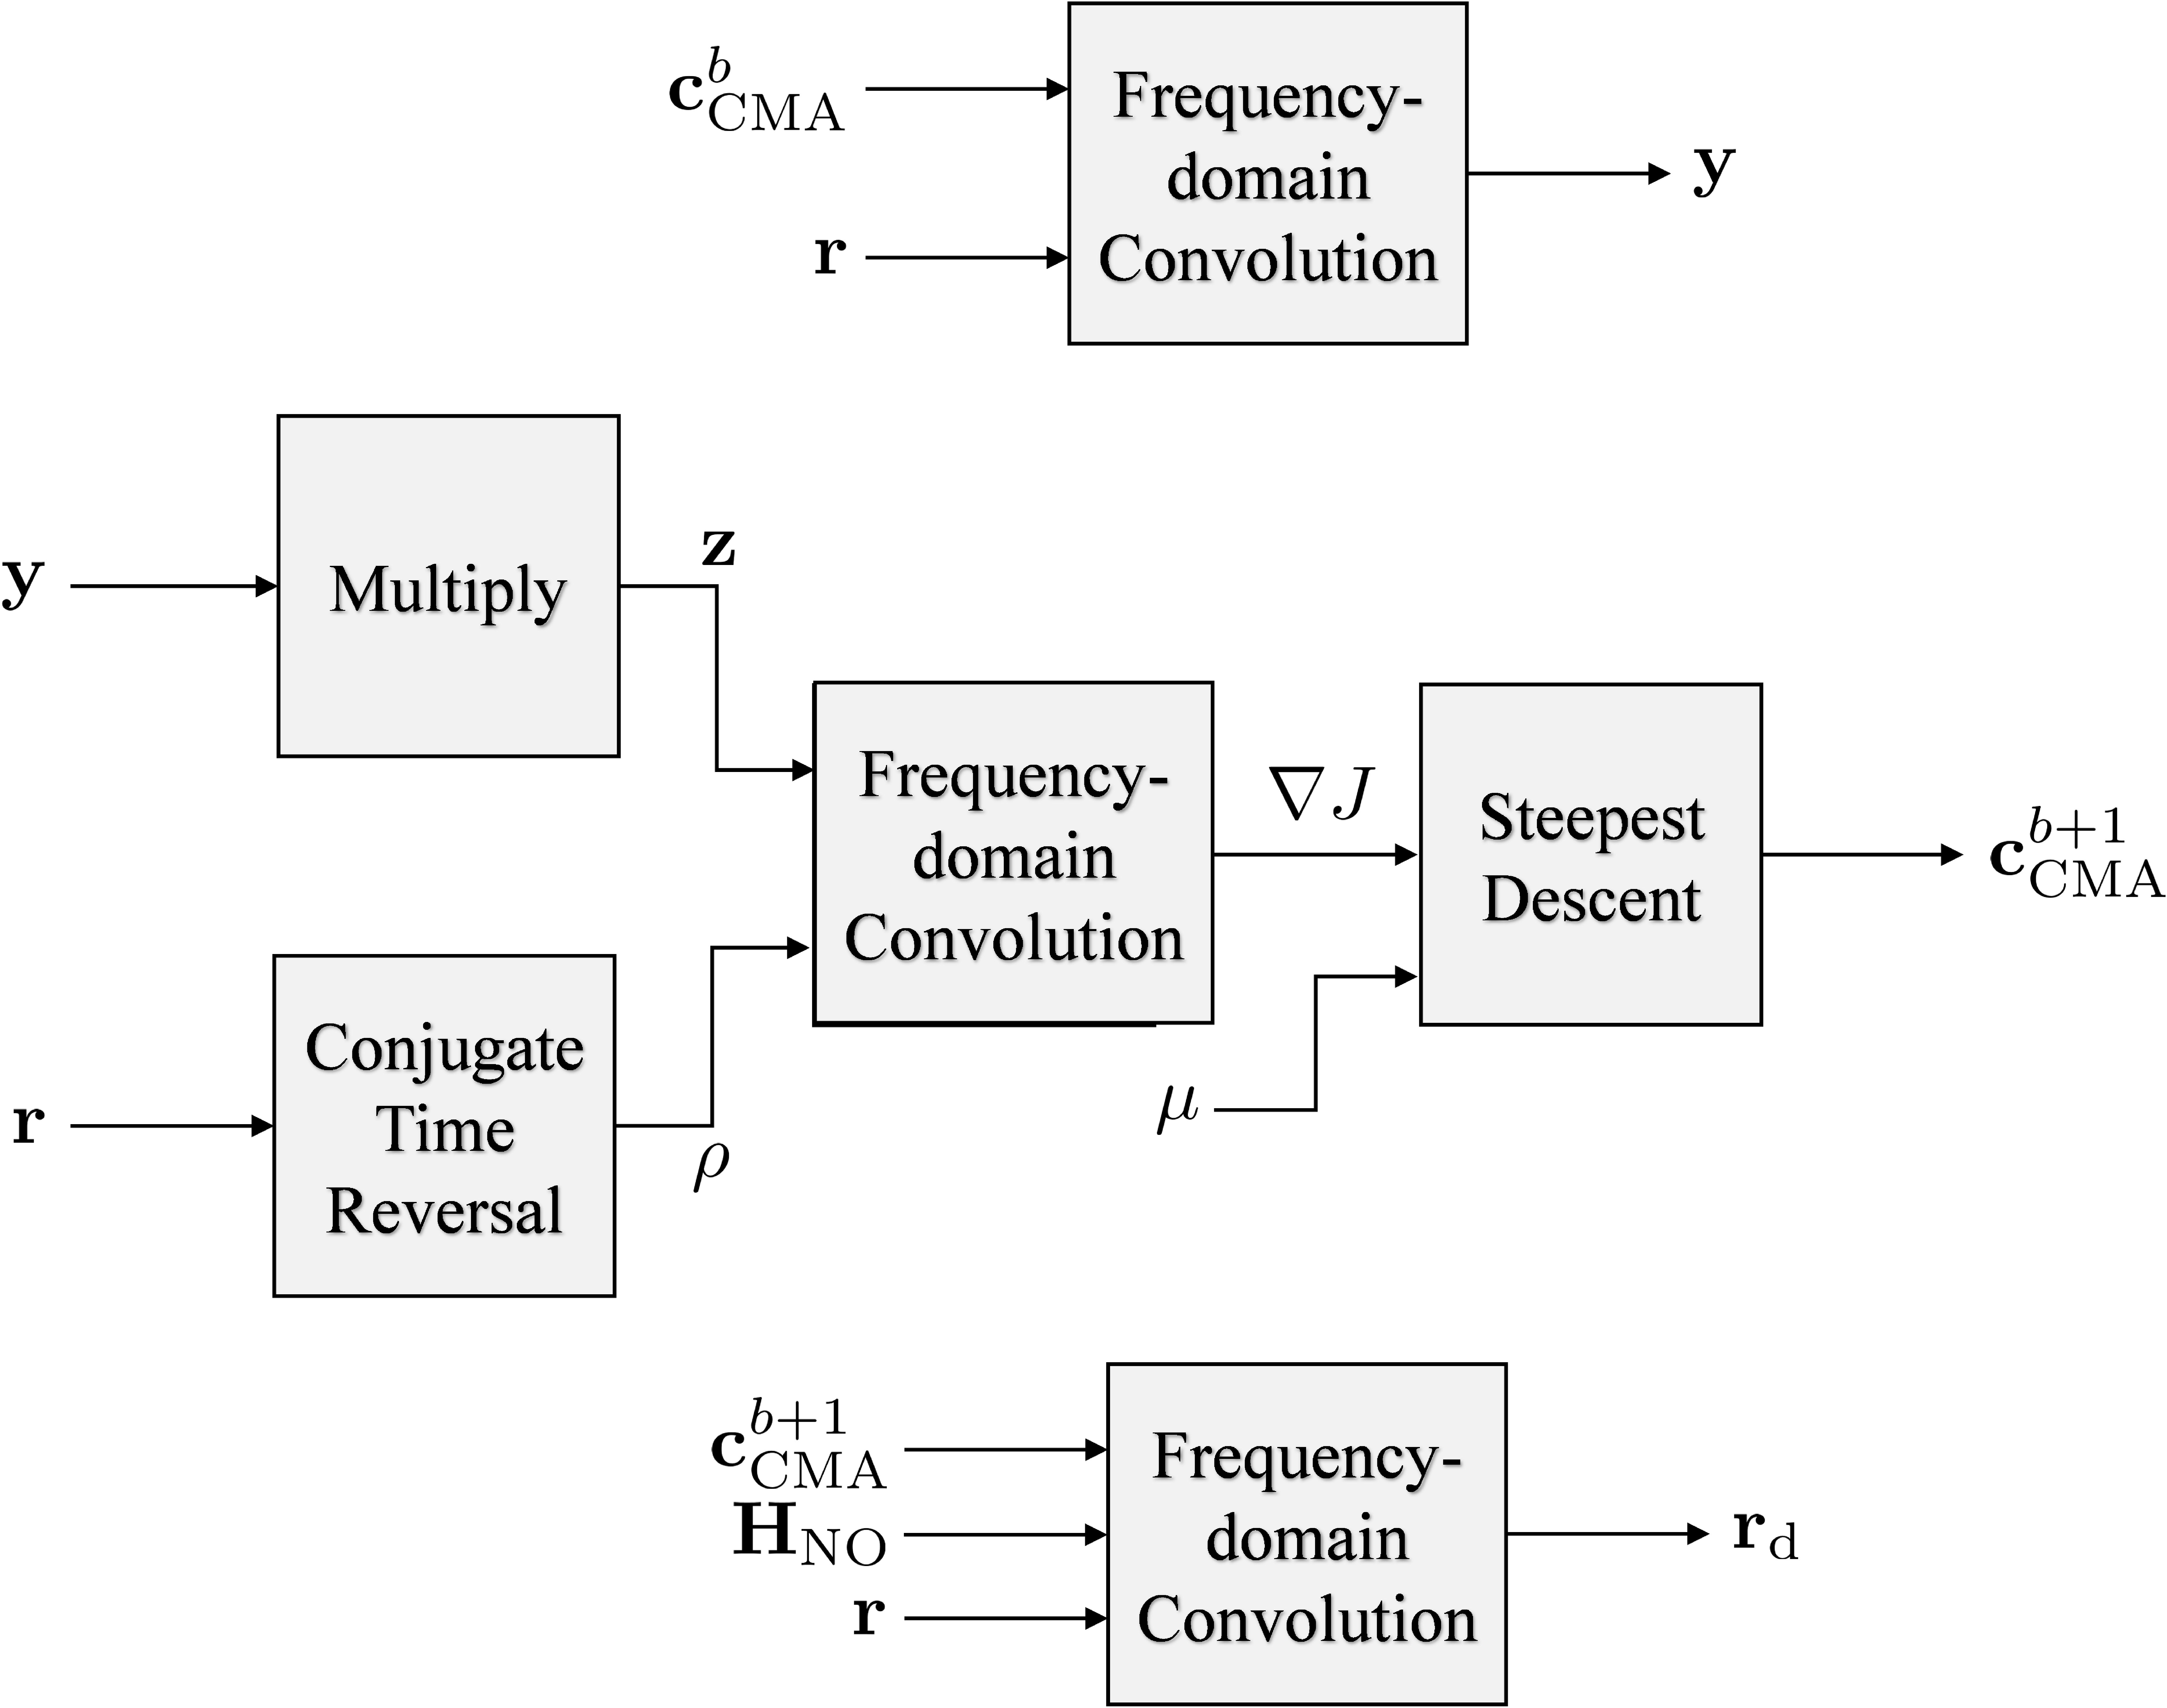
\includegraphics[width=10.68in/100*55]{figures/eq_GPUimplementation/blockCMA.pdf}
	\label{fig:blockCMA}
\end{figure}


\section{Frequency Domain Equalizer One and Two GPU Implementation}
The Frequency Domain Equalizers are by far the fastest and easiest to implement into GPUs.
Really, the block diagram looks just like convolution accept that hadamard product is replace with a different point to point multiply.
We are already applying the filters in the frequency domain...so lets just wrap the equalizer calculation and detection filter application together by
\begin{equation}
R_\text{d}(e^{j\omega_k}) = \frac{R(e^{j\omega_k}) \hat{H}^\ast(e^{j\omega_k})}  {|\hat{H}(e^{j\omega_k})|^2  +  \frac{1}{\hat{\sigma}^2_w}} \quad
\text{where} \;
\omega_k = \frac{2\pi}{L} \;
\text{for} \;
k=0,1,\cdots,L-1
\label{eq:FDE1_applied}
\end{equation}
or 
\begin{equation}
R_\text{d}(e^{j\omega_k}) = \frac{R(e^{j\omega_k}) \hat{H}^\ast(e^{j\omega_k})}  {|\hat{H}(e^{j\omega_k})|^2  +  \frac{\Psi(e^{j\omega_k})}{\hat{\sigma}^2_w}} \quad
\text{where} \;
\omega_k = \frac{2\pi}{L} \;
\text{for} \;
k=0,1,\cdots,L-1
\label{eq:FDE2_applied}
\end{equation}
where $R(e^{j\omega_k}$ and $R_\text{d}(e^{j\omega_k}$ is the FFT $\mathbf{r}$ and $\mathbf{r}_\text{d}$ 
at $\omega_k$.

\subsubsection{Frequency Domain Equalizer One}
\begin{figure}
	\caption{Diagram showing the relationships between $z(n)$, $\rho(n)$ and $b(n)$.}
	\centering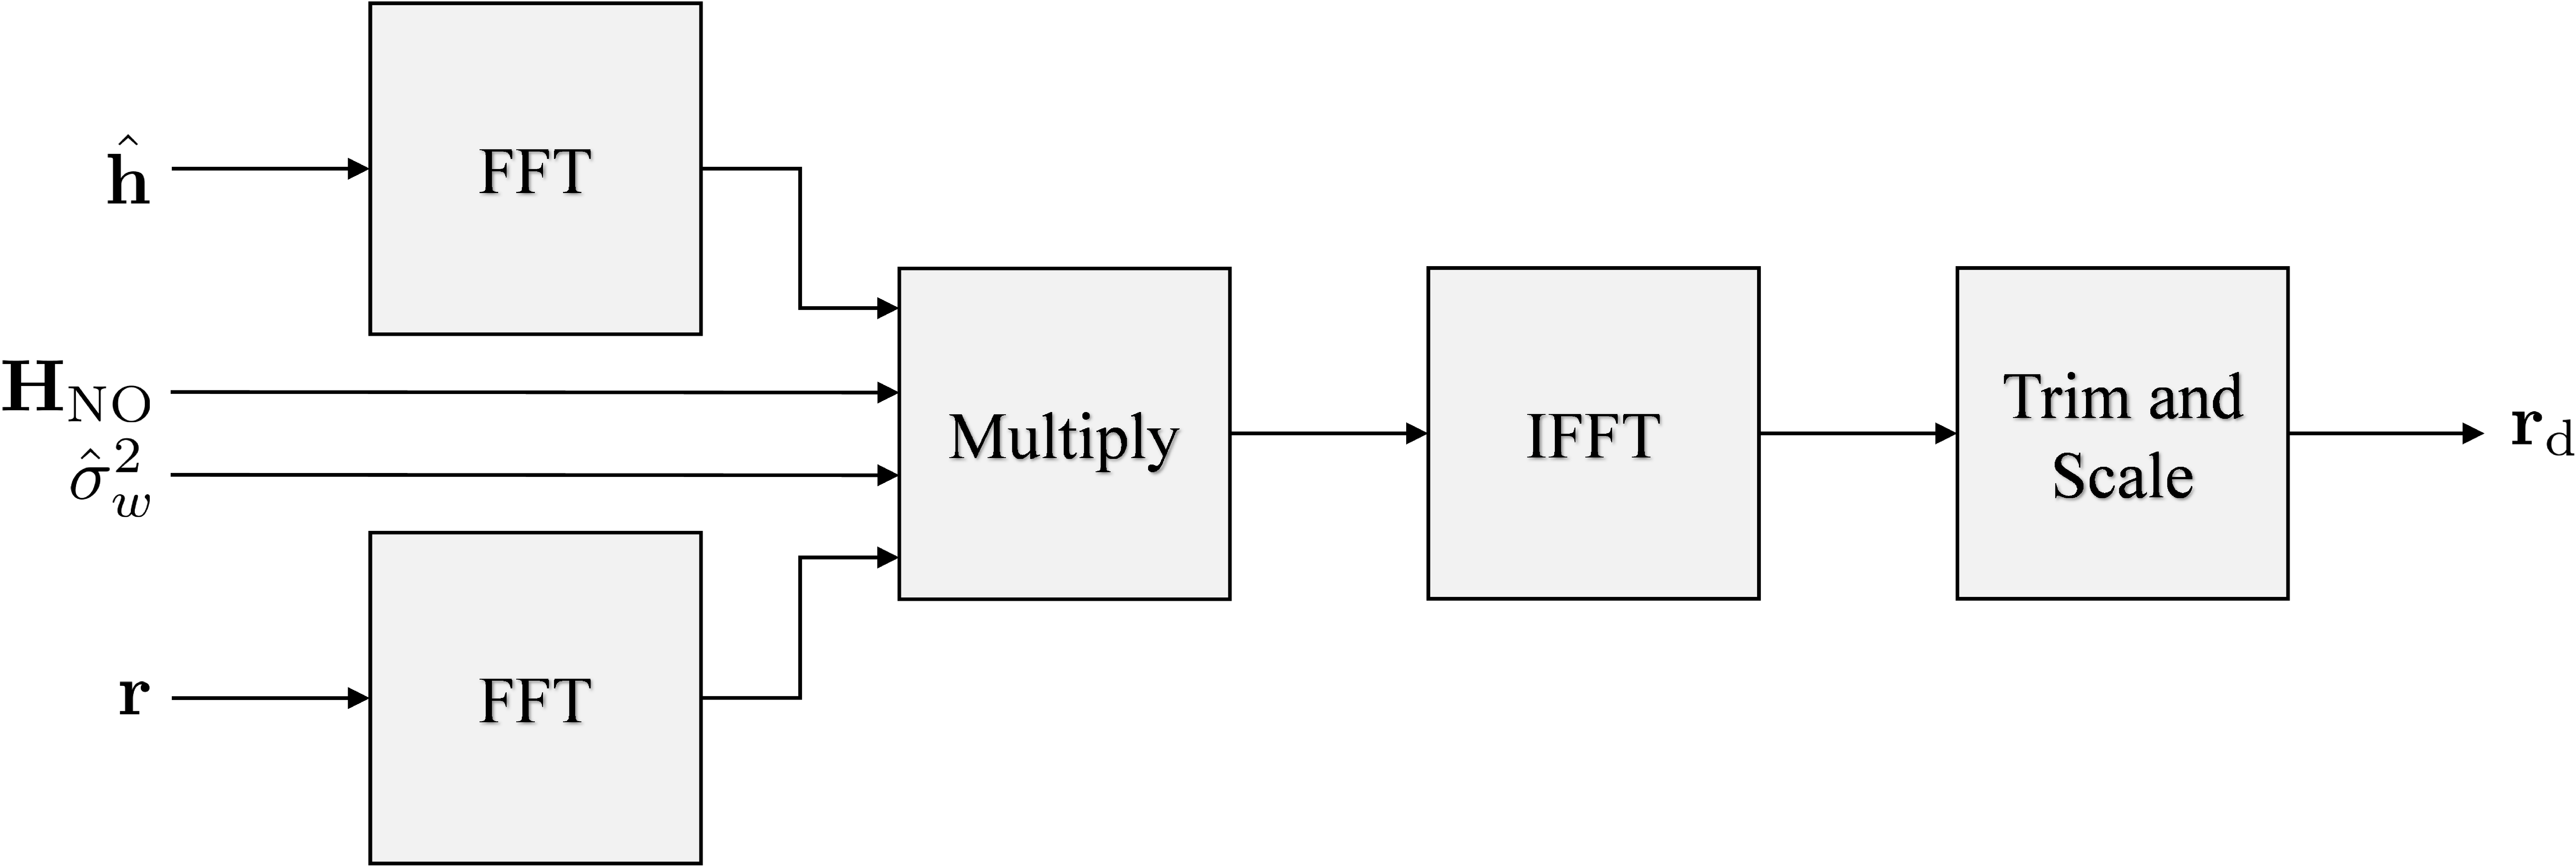
\includegraphics[width=9.73in/100*55]{figures/eq_GPUimplementation/blockFDE1.pdf}
	\label{fig:blockFDE1}
\end{figure}
\subsubsection{Frequency Domain Equalizer Two}
\begin{figure}
	\caption{Diagram showing the relationships between $z(n)$, $\rho(n)$ and $b(n)$.}
	\centering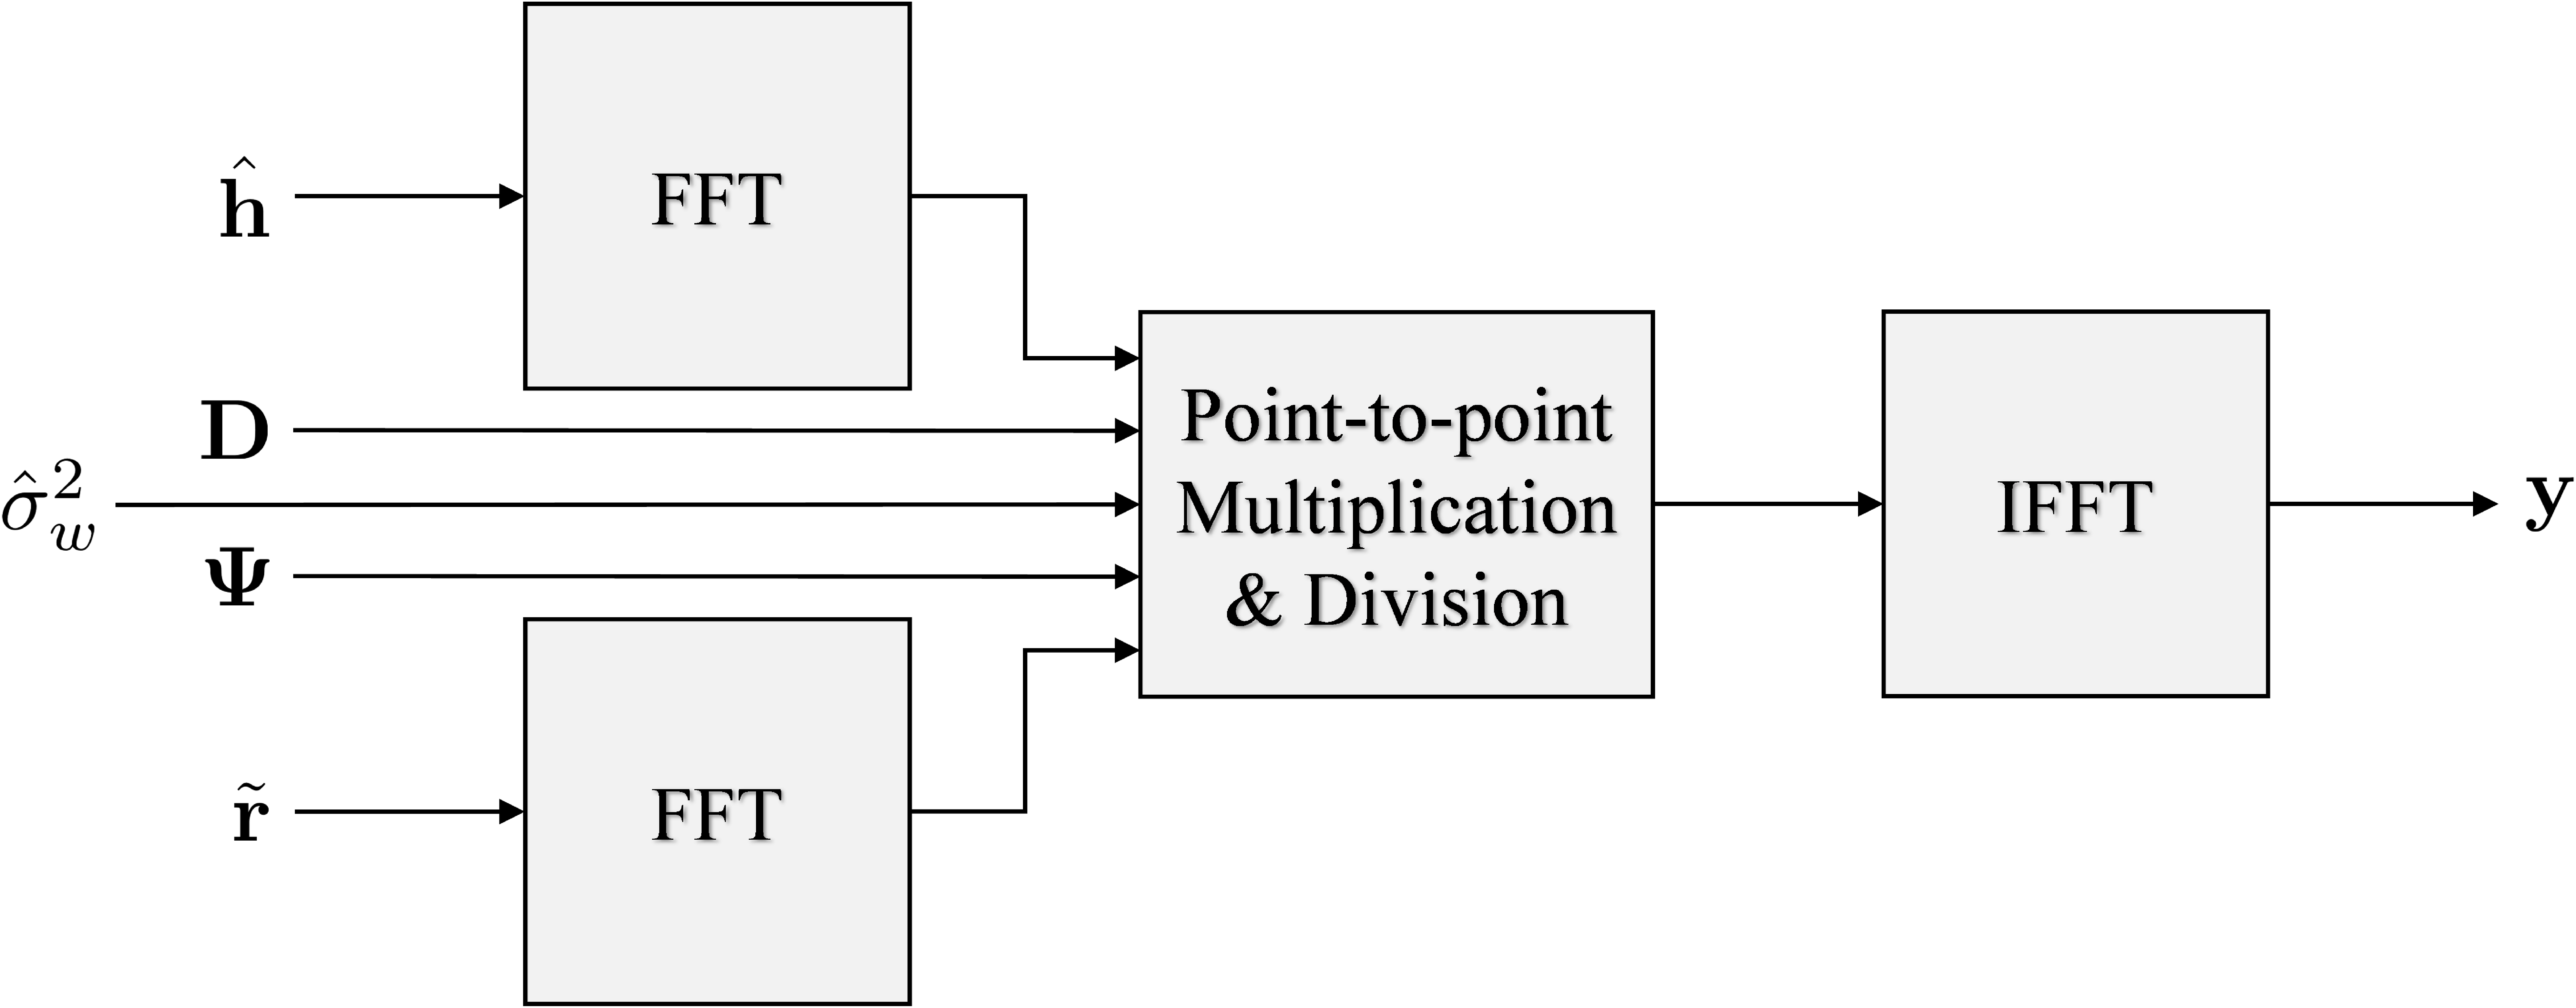
\includegraphics[width=10.03in/100*55]{figures/eq_GPUimplementation/blockFDE2.pdf}
	\label{fig:blockFDE2}
\end{figure}





